\label{ap:ap01}
\chapter{Introdução à Inteligência Artificial}

\section*{\textbf{A - ENUNCIADO}}

% \renewcommand{\thesubsection}{\arabic{subsection}}
% \makeatletter
% \renewcommand{\subsection}[1]{%
%   \refstepcounter{subsection}%
%   \vspace{1em}%
%   {\noindent\hspace{1em}\textbf{\thesubsection~#1}}%
%   \par
% }
% \makeatother

\subsection*{\textbf{1 ChatGPT}}
    \begin{enumerate}[label=\alph*)]
        \item \textbf{(6,25 pontos)} Pergunte ao ChatGPT o que é Inteligência Artificial e cole aqui o resultado.
        \item \textbf{(6,25 pontos)} Dada essa resposta do ChatGPT, classifique usando as 4 abordagens vistas em sala. Explique o porquê.
        \item \textbf{(6,25 pontos)} Pesquise sobre o funcionamento do ChatGPT (sem perguntar ao próprio ChatGPT) e escreva um texto contendo no máximo 5 parágrafos. Cite as referências.
        \item \textbf{(6,25 pontos)} Entendendo o que é o ChatGPT, classifique o próprio ChatGPT usando as 4 abordagens vistas em sala. Explique o porquê.
    \end{enumerate}

\subsection*{\textbf{2 Busca Heurística}}
    Realize uma busca utilizando o algoritmo A* para encontrar o melhor caminho para chegar a \textbf{Bucharest} partindo de \textbf{Lugoj}. Construa a árvore de busca criada pela execução do algoritmo apresentando os valores de $f(n)$, $g(n)$ e $h(n)$ para cada nó. Utilize a heurística de distância em linha reta, que pode ser observada na tabela abaixo.

    Essa tarefa pode ser feita em uma ferramenta de desenho, ou até mesmo no papel, desde que seja digitalizada (foto) e convertida para PDF.
    \begin{enumerate}[label=\alph*)]
        \item \textbf{(25 pontos)} Apresente a árvore final, contendo os valores, da mesma forma que foi apresentado na disciplina e nas práticas. Use o formato de árvore, não será permitido um formato em blocos, planilha, ou qualquer outra representação.
    \end{enumerate}

    \textbf{NÃO É NECESSÁRIO IMPLEMENTAR O ALGORITMO.}
    \begin{figure}[H]
        \centering
        \caption{Rotas Lugoj-Bucharest}
        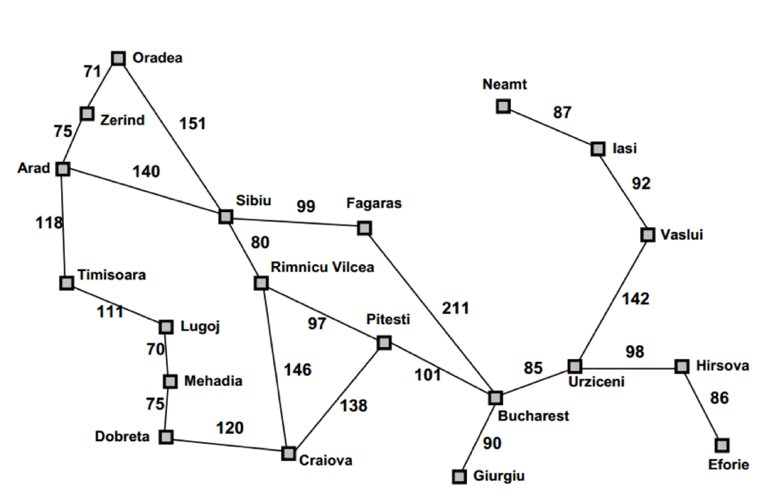
\includegraphics[width=0.7\textwidth]{apendices/fig/1_IAA001_1.png} 
        \caption*{Fonte: IAA UFPR (2025).}
        %\label{fig:minha_figura}
    \end{figure}
    \begin{figure}[H]
        \centering
        \caption{Distâncias em linha reta para a cidade de Bucharest}
        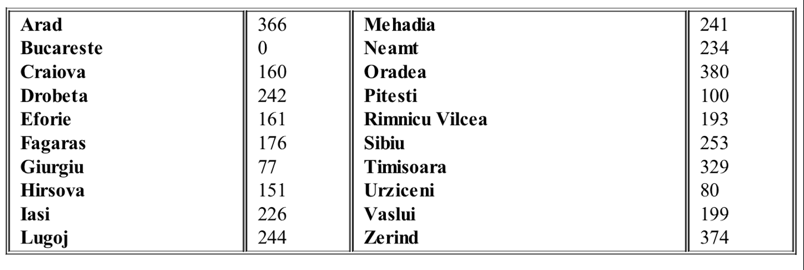
\includegraphics[width=0.7\textwidth]{apendices/fig/1_IAA001_2.png} 
        \caption*{Fonte: IAA UFPR (2025).}
        %\label{fig:minha_figura}
    \end{figure}

\subsection*{\textbf{3 Lógica}}
    Verificar se o argumento lógico é válido.

    \begin{adjustwidth}{3em}{}
        \begin{quote}
            \itshape
            Se as uvas caem, então a raposa as come \\
            Se a raposa as come, então estão maduras \\
            As uvas estão verdes ou caem

            Logo

            A raposa come as uvas se e somente se as uvas caem
        \end{quote}
    \end{adjustwidth}

    Deve ser apresentada uma prova, no mesmo formato mostrado nos conteúdos de aula e nas práticas.

    \begin{adjustwidth}{1em}{}
    \textbf{Dicas:}
    \end{adjustwidth}
    \begin{enumerate}[label=\arabic*.]
        \item Transformar as afirmações para lógica:

        $p$: as uvas caem \\
        $q$: a raposa come as uvas \\
        $r$: as uvas estão maduras

        \item Transformar as três primeiras sentenças para formar a base de conhecimento

        R1: $p \rightarrow q$ \\
        R2: $q \rightarrow r$ \\
        R3: $\neg r \vee p$

        \item Aplicar equivalências e regras de inferência para se obter o resultado esperado. Isto é, com essas três primeiras sentenças devemos derivar $q \leftrightarrow p$. Cuidado com a ordem em que as fórmulas são geradas.

        \textbf{Equivalência Implicação:} $(\alpha \rightarrow \beta)$ equivale a $(\neg \alpha \vee \beta)$

        \textbf{Silogismo Hipotético:} $\alpha \rightarrow \beta$, $\beta \rightarrow \gamma \vdash \alpha \rightarrow \gamma$

        \textbf{Conjunção:} $\alpha$, $\beta \vdash \alpha \wedge \beta$

        \textbf{Equivalência Bicondicional:} $(\alpha \leftrightarrow \beta)$ equivale a $(\alpha \rightarrow \beta) \wedge (\beta \rightarrow \alpha)$
    \end{enumerate}

    \begin{enumerate}[label=\alph*)]
        \item \textbf{(25 pontos)} Deve-se mostrar todos os passos e regras aplicadas, no mesmo formato apresentado nas aulas e nas práticas. As equivalências e regras necessárias estão descritas acima e no material.
    \end{enumerate}

\subsection*{\textbf{4 Redes Neurais Artificiais}}
    Seja a RNA da figura abaixo.
    
    \begin{figure}[H]
        \centering
        \caption{Rede Neural Artificial exercício 4}
        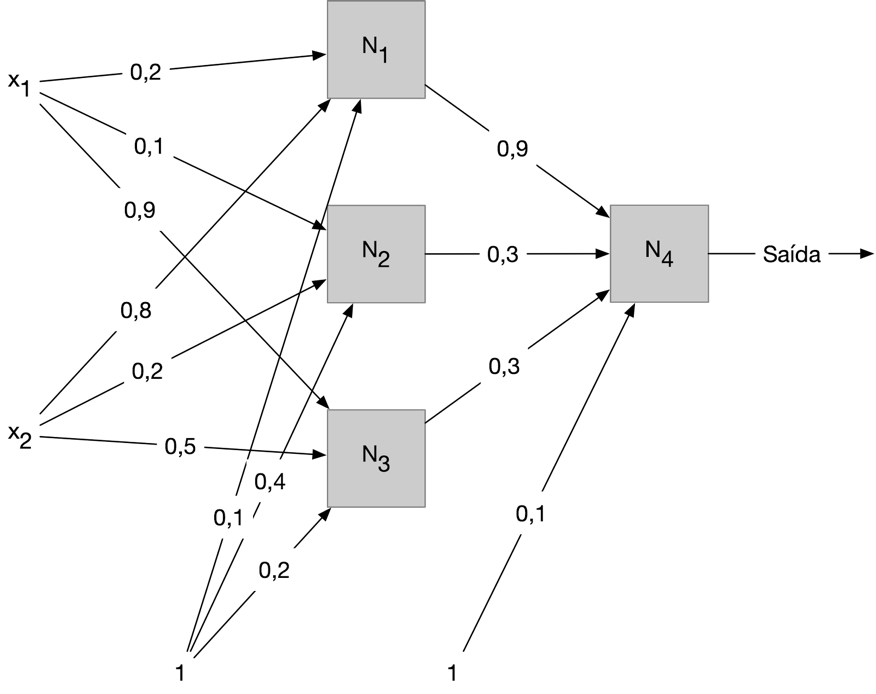
\includegraphics[width=0.7\textwidth]{apendices/fig/1_IAA001_3.png} 
        \caption*{Fonte: IAA UFPR (2025).}
        %\label{fig:minha_figura}
    \end{figure}

    Os neurônios $N_1$, $N_2$ e $N_3$ possuem função de ativação linear. Já $N_4$ possui função de ativação tangente hiperbólica (pesquise a fórmula e aplique).

    Dada a entrada $x_1 = -3$, $x_2 = 1$, dê:
    \begin{enumerate}[label=\alph*)]
        \item \textbf{(6,25 pontos)} Valor de saída do neurônio N1
        \item \textbf{(6,25 pontos)} Valor de saída do neurônio N2
        \item \textbf{(6,25 pontos)} Valor de saída do neurônio N3
        \item \textbf{(6,25 pontos)} Valor de saída da rede como um todo
    \end{enumerate}

\section*{\textbf{B - RESOLUÇÃO}}
\setcounter{subsection}{0}

\subsection*{\textbf{1 ChatGPT}}
\begin{adjustwidth}{1em}{}
\textbf{a) Pergunte ao ChatGPT o que é Inteligência Artificial e cole aqui o resultado.}
\end{adjustwidth}

Inteligência Artificial (IA) refere-se à capacidade de um sistema ou programa de computador realizar tarefas que normalmente exigiriam inteligência humana. Essas tarefas incluem raciocínio, aprendizado, percepção visual, reconhecimento de fala, compreensão de linguagem natural, tomada de decisões e resolução de problemas.

Os sistemas de IA são projetados para imitar certos aspectos da inteligência humana, utilizando algoritmos e modelos matemáticos para processar dados, aprender padrões e tomar decisões. Existem dois tipos principais de IA:

\begin{enumerate}
    \item IA Fraca (ou Estreita): Refere-se a sistemas de IA especializados em tarefas específicas. Eles são limitados ao escopo de suas programações e não têm a capacidade de realizar tarefas além do que foram projetados para fazer. Exemplos incluem reconhecimento de voz, chatbots e carros autônomos.
    \item IA Forte (ou Geral): Envolve sistemas que têm a capacidade de realizar qualquer tarefa cognitiva que um ser humano pode fazer. Este nível de IA ainda não foi totalmente alcançado e é um campo de pesquisa em desenvolvimento.
\end{enumerate}
    
Algoritmos de aprendizado de máquina (Machine Learning) são frequentemente usados na implementação de sistemas de IA. Eles permitem que a IA melhore seu desempenho em uma tarefa específica à medida que é exposta a mais dados, sem ser explicitamente programada.

A Inteligência Artificial tem aplicações em uma variedade de setores, como medicina, finanças, automação industrial, reconhecimento de padrões, entretenimento e muito mais. É uma área de rápido avanço e continua a desempenhar um papel significativo na transformação de várias indústrias.

\begin{adjustwidth}{1em}{}
\textbf{b) Dada essa resposta do ChatGPT, classifique usando as 4 abordagens vistas em
sala. Explique o porquê.}
\end{adjustwidth}

A definição dada pelo ChatGPT menciona que sistemas de Inteligência Artificial são projetados para "imitar certos aspectos da inteligência humana", o que parece se assemelhar mais à definição de Pensar como Humanos ou Agir como Humanos.

\begin{adjustwidth}{1em}{}
\textbf{c) Pesquise sobre o funcionamento do ChatGPT (sem perguntar ao próprio
ChatGPT) e escreva um texto contendo no máximo 5 parágrafos. Cite as referências.}
\end{adjustwidth}

O ChatGPT pode se entendido como uma extrapolação de uma classe de modelos de aprendizagem de máquina chamados Large Language Models (LLMs), que são modelos de Processamento de Linguagem Natural. Esse tipo de modelo consegue processar grandes quantidades de texto e inferir relações entre palavras dentro do texto. A capacidade dos LLMs cresce conforme aumenta o tamanho e variedade de parâmetros da base de dados.\cite{towardsdatascience}

Segundo o que é disponibilidado pelo OpenAI\cite{OpenAI}, ele é baseado na arquitetura GPT (Generative Pre-trained Transformer), um modelo Transformer, que é uma rede neural capaz de aprender o contexto dado e gerar um novo texto a partir disso. A rede foi otimizada para usar um método de treinamento chamado Reinforcement Learning with Human Feedback (RLHF), que usa demonstrações humanas para guiar seu comportamento, de forma a alcançar o desejável.

Segundo Rama Ramakrishnan, professor do MIT, \cite{MIT}, o modelo precedente, GPT-3, foi treinado com cerca de 30 bilhões de frases retiradas de livros e da internet, para uma única tarefa: prever a palavra seguinte em uma frase, dadas as palavras usadas anteriormente. Ele calcula uma tabela de probabilidades para possíveis palavras a serem usadas e usa a que tem a melhor probabilidade, quase como um sistema de \textit{autocomplete}. Para formar frases completas, a cada palavra escolhida, ele adiciona ela à frase e refaz o processo de cálculo das probabilidades para escolher a próxima palavra. Já a versão 3.5 foi treinada para seguir instruções dadas por humanos, utilizando uma base de dados contendo pares de exemplos de instruções e respostas de alta qualidade para tais instruções. O modelo treinado a partir dessa base de dados foi então utilizado para gerar múltiplas respostas para cada uma das instruções e essas respostas foram categorizadas por humanos de mais útil a menos útil. A partir desses novos dados, foi possível treinar um "modelo de recompensa", que avalia a qualidade das respostas geradas pelo GPT-3.5 e retorna uma "nota" de avaliação para o GPT-3.5, assim ele passa por um \textit{fine tuning} para melhorar suas respostas com \textit{reinforcement learning}. Na transição do GPT-3.5 para o ChatGPT foi usado um processo similar, mas desta vez utilizando conversas inteiras para o treinamento.

Ele é treinado usando textos escritos por humanos, incluindo conversações, de forma a conseguir imitar o estilo de comunicação humano). Assim, de acordo com os dados utilizados para treinamento, ele pode, inclusive, produzir textos com conteúdo enviesado.

\begin{adjustwidth}{1em}{}
\textbf{d) Entendendo o que é o ChatGPT, classifique o próprio ChatGPT usando as 4
abordagens vistas em sala. Explique o porquê.}
\end{adjustwidth}

De acordo com o comportamento, que se baseia em aprender e imitar como humanos se comunicam, ele parece se encaixar na definição da abordagem Agir como Humanos. Essa conclusão pode ser atingida considerando-se que o ChatGPT encontra padrões nos textos, que são dados produzidos (majoritariamente) por humanos, e com isso aprende contextos, mas não é totalmente consciente sobre o seu conteúdo, e não usa um processo cognitivo, apenas os sintetiza conforme foram fornecidos a ele. Como exemplo, se o ChatGPT fosse treinado com textos com um viés racista, ele poderia reproduzir textos racistas, já que não tem a capacidade de ponderar se racismo é correto ou não de um ponto de vista racional, ou seja, ele não toma decisões racionais baseadas no contexto que é apresentado a ele, apenas busca imitar a forma como humanos se comunicam.

\subsection*{\textbf{2 Busca Heurística}}
%\begin{figure}[H]
%\centering
%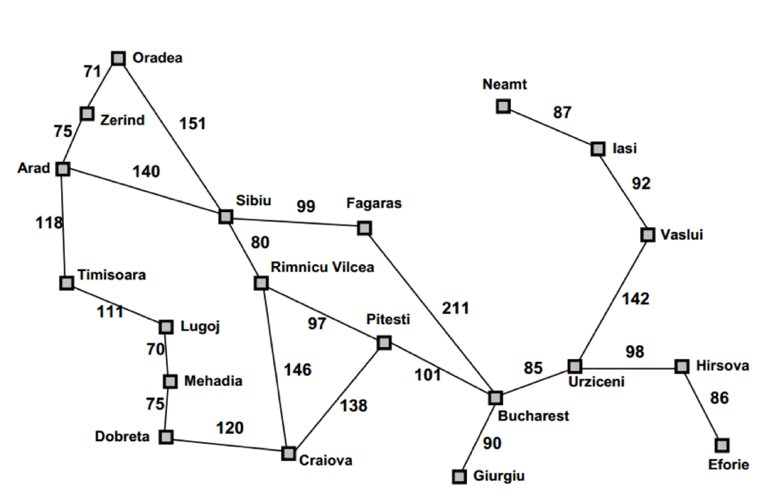
\includegraphics[width=0.6\linewidth]{apendices/fig/1_IAA001_1.png}
%\caption{Rotas Lugoj-Bucharest}
%\label{grafoAStar}
%\end{figure}

\begin{adjustwidth}{1em}{}
\textbf{a) Apresente a árvore final, contendo os valores, da mesma forma que foi apresentado
na disciplina e nas práticas. Use o formato de árvore, não será permitido um formato em blocos,
planilha, ou qualquer outra representação.}
\end{adjustwidth}

\begin{figure}[H]
\centering
\caption{Árvore final}
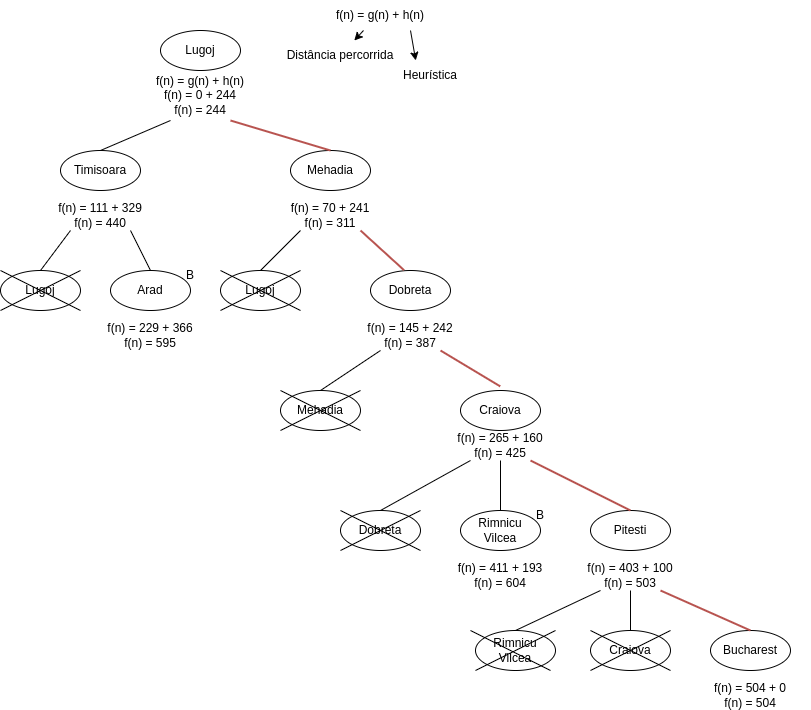
\includegraphics[width=0.8\linewidth]{apendices/fig/1_IAA001_4.png}
\caption*{Fonte: O autor (2025).}
\label{arvoreF}
\end{figure}

$Lugoj \Rightarrow Mehadia \Rightarrow Dobreta \Rightarrow Craiova \Rightarrow Pitesti \Rightarrow Bucharest$ = 504

\subsection*{\textbf{3 Lógica}}
\begin{adjustwidth}{3em}{}
\begin{quote}
    \itshape
    Se as uvas caem, então a raposa as come \\
    Se a raposa as come, então estão maduras \\
    As uvas estão verdes ou caem

    Logo

    A raposa come as uvas se e somente se as uvas caem
\end{quote}
\end{adjustwidth}

$p$: as uvas caem 

$q$: a raposa come as uvas 

$r$: as uvas estão maduras

\begin{equation*}
    \begin{gathered}
        R1: p \Rightarrow q \\
        R2: q \Rightarrow r \\
        R3: \neg{r} \lor p \\
    \end{gathered}
\end{equation*}

objetivo: 
\begin{equation*}
    q \Leftrightarrow p
\end{equation*}

%ou seja, aplicando a Equivalência Bicondicional:

%\begin{equation*}
%    p \Rightarrow q \ e \ q \Rightarrow p
%\end{equation*}

\begin{adjustwidth}{1em}{}
\textbf{a) Deve-se mostrar todos os passos e regras aplicadas, no mesmo formato
apresentado nas aulas e nas práticas.}
\end{adjustwidth}

%Como a primeira afirmação lógica necessária para a prova já está na base de conhecimento (R1), para que a equivalência acima seja verdadeira, é necessário provar que:

%\begin{equation*}
%    q \Rightarrow p
%\end{equation*}

%Partindo da base de conhecimento:

% de \ R1 \ e \ R2:
% \begin{equation}
%     R4: p \Rightarrow r \\
% \end{equation}

%usando Equivalência Implicação em R3 temos:

\begin{equation*}
    \begin{gathered}
        R1: p \Rightarrow q \\
        R2: q \Rightarrow r \\
        R3: \neg{r} \lor p \\
    \end{gathered}
\end{equation*}

%\hrule

\begin{align*}
    R4: r \Rightarrow p && \text{Equivalência Implicação, R3 }
\end{align*}
%usando Silogismo Hipotético em R2 e R4, temos que:
\begin{align*}
    R5: q \Rightarrow p && \text{SH, R2, R4 }
\end{align*}
\begin{align*}
    R6: p \Rightarrow q \land q \Rightarrow p && \text{CONJ, R1, R5 }
\end{align*}
\begin{align*}
    R7: q \Leftrightarrow p && \text{BICOND, R6 }
\end{align*}

%concluindo assim a prova lógica.

\subsection*{\textbf{4 Redes Neurais Artificiais}}

x1=-3, x2=1

N1, N2, N3: função de ativação linear (mantém o valor)

N4: função de ativação tangente (produz valores no intervalo [-1,1])

\begin{figure}[!h]
\centering
\caption{Tangente Hiperbólica}
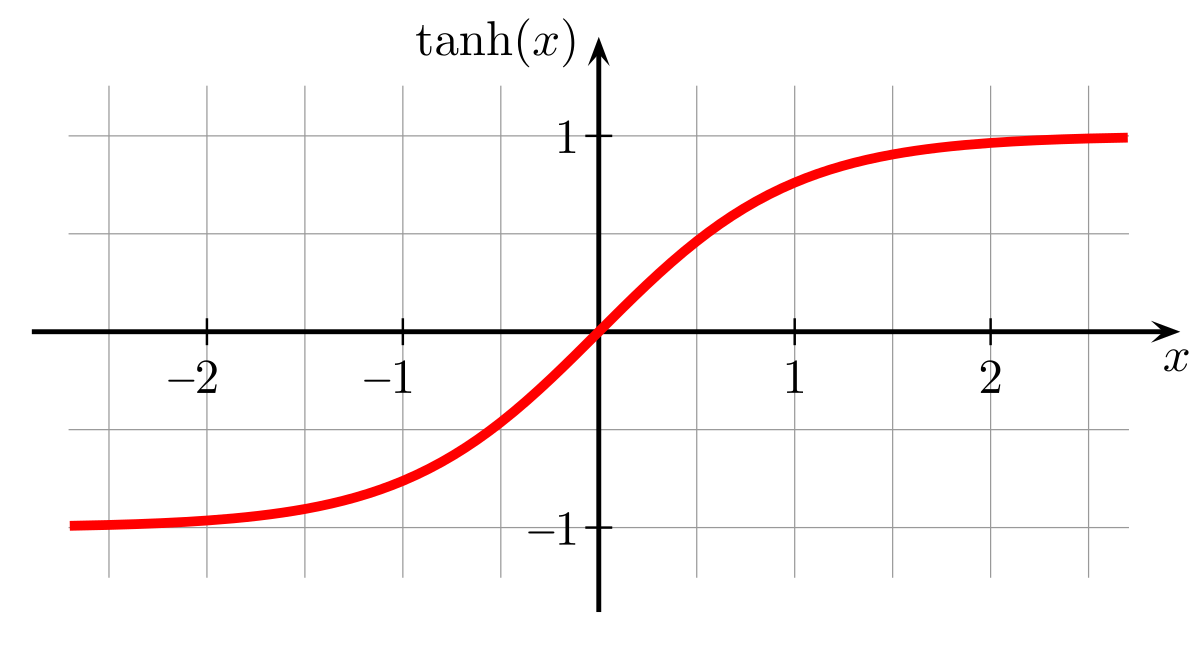
\includegraphics[width=0.6\linewidth]{apendices/fig/1_IAA001_5.png}
\caption*{Fonte: O autor (2025).}
\label{tanh}
\end{figure}

%\begin{figure}[H]
%\centering
%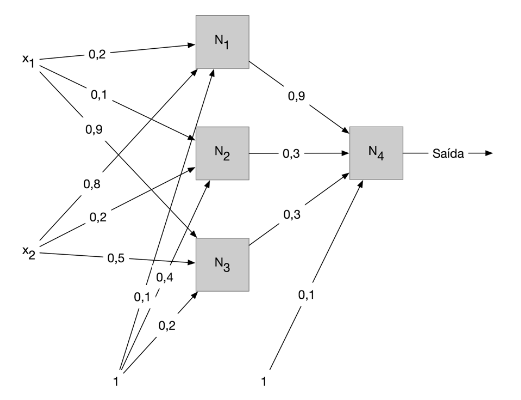
\includegraphics[width=0.6\linewidth]{apendices/fig/1_IAA001_6.png}
%\caption{Rede Neural Artificial exercício 4}
%\label{rede}
%\end{figure}

\begin{adjustwidth}{1em}{}
\textbf{a) Valor de saída do neurônio N1}
\end{adjustwidth}
\begin{equation*}
    (-3)\times0.2 + 1\times0.8 + 1\times0.1 = 0.3
\end{equation*}

\begin{adjustwidth}{1em}{}
\textbf{b) Valor de saída do neurônio N2}
\end{adjustwidth}
\begin{equation*}
    (-3)\times0.1 + 1\times0.2 + 1\times0.4 = 0.3
\end{equation*}

\begin{adjustwidth}{1em}{}
\textbf{c) Valor de saída do neurônio N3}
\end{adjustwidth}
\begin{equation*}
    (-3)\times0.9 + 1\times0.5 + 1\times0.2 = -2
\end{equation*}

\begin{adjustwidth}{1em}{}
\textbf{d) Valor de saída da rede como um todo}
\end{adjustwidth}
\begin{equation*}
    tanh(0.3\times0.9 + 0.3\times0.3 + (-2)\times0.3 + 1\times0.1) = tanh(0.27 + 0.09 - 0.6 + 0.1) = -0.13909 \approx -0.14
\end{equation*}